\documentclass[10pt,a4paper,twocolumn]{article}

\usepackage[margin=0.75in,columnsep=0.3in]{geometry}
\usepackage{amsmath, amssymb, amsthm}
\usepackage{graphicx}
\usepackage{hyperref}
\usepackage{enumitem}
\usepackage{booktabs}
\usepackage{caption}
\usepackage{xcolor}
\usepackage{listings}
\usepackage{multirow}
\usepackage{array}
\usepackage{makecell}
\usepackage{titling}
\usepackage{tikz}
\usetikzlibrary{positioning,arrows.meta,shapes.geometric,fit,backgrounds}

% Tighten lists in two-column
\setlist{topsep=2pt,itemsep=2pt,parsep=0pt}

\lstset{
  basicstyle=\ttfamily\footnotesize,
  keywordstyle=\color{blue},
  commentstyle=\color{gray},
  stringstyle=\color{red!70!black},
  breaklines=true,
  frame=single,
  numbers=left,
  numberstyle=\tiny\color{gray},
  language=Python
}

\hypersetup{
  colorlinks=true,
  linkcolor=black,
  citecolor=blue!60!black,
  urlcolor=blue!60!black
}

% Captions tighter
\captionsetup{font=small,labelfont=bf,skip=4pt}

% Title block (two-column papers normally span title across both columns)
\title{\vspace{-0.3in}\Large\textbf{Modern Retrieval-Augmented Discovery of RESTful Web APIs:
Empirically Reassessing the Need for LLM Hierarchical Reasoning}\\[0.4em]
\large\normalfont Mini-Project Report --- Department of Computer Science and Engineering}

% Plain \author block — avoids authblk conflict with @twocolumnfalse
\author{%
  \large Aman Kumar (cs23b1003@iiitr.ac.in) \quad\textnormal{and}\quad Rudra Pratap Singh (ad23b1047@iiitr.ac.in) \\[0.5em]
  \normalsize Indian Institute of Information Technology, Raichur \\[0.2em]
  \normalsize \textit{Project Supervisor:} \textbf{Dr.\ Neha Agarwal}
}
\date{May 2026}

\begin{document}

% Twocolumn-friendly title spanning both columns
\twocolumn[
\begin{@twocolumnfalse}
  \maketitle
  \vspace{-1em}
  \begin{abstract}
  \noindent
  Discovering the right RESTful Web API among the tens of thousands published
  on contemporary marketplaces is a real productivity bottleneck for software
  developers. The recent paper of Li, Ai, Kang, Qiu and Liu (\emph{Service
  Oriented Computing and Applications}, 2025) addresses this with a
  three-level hierarchical Large Language Model (LLM) prompting framework on
  the RapidAPI platform, augmented with a heuristic self-checking mechanism,
  and reports a GPT-4 hierarchical pipeline as the strongest configuration.
  In this work we empirically reassess the necessity of that LLM hierarchical
  machinery. We implement a two-phase pipeline that pairs a strong modern
  dense embedder (\texttt{BGE-large-en-v1.5}) with classical lexical retrieval
  (BM25) under Reciprocal Rank Fusion, and then adds Hypothetical Document
  Embeddings (HyDE) together with a 568M-parameter cross-encoder reranker
  (\texttt{BGE-reranker-v2-m3}). On a public RapidAPI proxy corpus of
  47{,}592 endpoints across 49 categories and a 50-query test set
  constructed by the paper's exact protocol, our Phase~1 retrieval-only
  pipeline already matches the paper's GPT-4 hierarchical \emph{Hit@20} score
  of 0.74 with zero LLM reasoning calls; our Phase~2 cross-encoder pipeline
  beats the paper's strongest configuration on five of six standard metrics,
  achieving \emph{Hit@5}=0.72 (paper: 0.60) and \emph{Hit@20}=0.80 (paper:
  0.74) at roughly fifty times lower per-query cost. We frame the remaining
  \emph{MRR@20} gap as a structurally explained phenomenon and outline a
  follow-on Phase~3 design that recovers it.

  \vspace{0.4em}
  \noindent\textbf{Keywords:} RESTful Web API, service discovery, dense
  retrieval, BM25, BGE, HyDE, cross-encoder reranking, large language
  models, RapidAPI.
  \end{abstract}
  \vspace{0.6em}
\end{@twocolumnfalse}
]

\section{Introduction}\label{sec:intro}

The number of public RESTful Web APIs has grown nearly an order of magnitude
in the past decade. RapidAPI alone hosts more than \textbf{40{,}000
endpoints} across roughly fifty categories~\cite{li2025llm}; ProgrammableWeb
listed about \textbf{24{,}000 APIs} before its 2022 shutdown; a single
platform such as Shopify exposes around \textbf{6{,}000 parameters} across
its endpoints. This abundance is a blessing for developers who can now
compose applications from existing services rather than implementing them
from scratch, but it has also created a new problem: \emph{discovering}
which API satisfies a given requirement is itself a non-trivial information
retrieval task.

Early service discovery research targeted SOAP/UDDI registries with
ontology-based and keyword-driven matching~\cite{paolucci2002,zhou2008}. The
shift to lightweight RESTful APIs --- usually documented in plain natural
language rather than formal description languages --- broke many of those
techniques. Recent work has therefore converged on three families of
approaches:
\begin{itemize}[leftmargin=*]
    \item \textbf{Lexical / sparse retrieval}, exemplified by BM25, which
          scores query--document pairs based on term overlap statistics.
    \item \textbf{Semantic / dense retrieval}, in which neural encoders
          such as Sentence-BERT~\cite{reimers2019sbert} or Dense Passage
          Retrieval (DPR)~\cite{karpukhin2020dpr} embed queries and
          documents into a shared vector space.
    \item \textbf{Large-language-model-mediated discovery}, in which a
          generative LLM~\cite{gpt4tr} is prompted to reason over a
          candidate set, sometimes hierarchically~\cite{li2025llm}.
\end{itemize}

The most prominent recent contribution along the third axis is the work of
Li \textit{et al.}~\cite{li2025llm} (\emph{Service Oriented Computing and
Applications}, November 2025). They propose a three-level hierarchical
prompt structure for service discovery on RapidAPI:
\emph{category-level}, \emph{API-level}, and \emph{endpoint-level},
augmented with a self-checking mechanism that asks the LLM two yes/no
questions per candidate API and applies a fixed score adjustment of
$+20$, $-10$, or $+10$. Their best configuration --- GPT-4 with
self-checking --- reaches \emph{Hit@20}=0.74 and \emph{MRR@20}=0.6773
on a 50-query test set drawn from RapidAPI.

Two empirical questions are left open by their study:
\begin{enumerate}[leftmargin=*]
    \item How much of the reported gain is attributable to the LLM's
          \emph{hierarchical reasoning}, and how much would simply follow
          from using a 2023-vintage dense embedder~\cite{xiao2023cpack}
          and a modern cross-encoder reranker~\cite{nogueira2019passage}
          instead of the paper's 2019-era
          Sentence-BERT~\cite{reimers2019sbert} baseline?
    \item Is the heuristic $+20/-10$ self-checking adjustment learnable
          from a cross-encoder probability, replacing the magic numbers
          with a principled signal?
\end{enumerate}
The present report addresses the first question directly and lays the
groundwork for the second.

\subsection{Contributions}

\begin{enumerate}[leftmargin=*]
    \item \textbf{A faithful reproduction protocol on a public corpus.}
          Since the paper's RapidAPI snapshot is not released, we use
          \texttt{stabletoolbench/ToolEnv2404}~\cite{stabletoolbench2024}
          --- a public RapidAPI dump of 47{,}592 endpoints across 49
          categories --- and reconstruct the paper's 50-query evaluation
          protocol end-to-end.
    \item \textbf{Phase~1 --- modern hybrid retrieval.} BM25 plus
          \texttt{BGE-large-en-v1.5}~\cite{xiao2023cpack} fused with
          Reciprocal Rank Fusion~\cite{cormack2009rrf} matches the
          paper's \emph{Hit@20}=0.74 with \emph{zero} LLM reasoning calls.
    \item \textbf{Phase~2 --- HyDE plus cross-encoder reranking.} Adding
          Hypothetical Document Embeddings~\cite{gao2023hyde} and the
          \texttt{BGE-reranker-v2-m3}~\cite{xiao2023cpack} cross-encoder
          beats the paper's GPT-4 hierarchical configuration on five of
          six metrics: \emph{Hit@5} 0.72 vs.\ 0.60, \emph{Hit@10} 0.78
          vs.\ 0.66, \emph{Hit@20} 0.80 vs.\ 0.74, \emph{MRR@5} 0.574
          vs.\ 0.507, \emph{MRR@10} 0.581 vs.\ 0.567.
    \item \textbf{An honest accounting of where we still trail.} The
          paper retains a \emph{MRR@20} edge (0.677 vs.\ our 0.582)
          traceable to ten queries that retrieval misses entirely; we
          propose a well-defined Phase~3 LLM hierarchical fallback over
          our pre-filtered top-100 candidates to recover those.
\end{enumerate}

\section{Background and Motivation}\label{sec:background}

\subsection{The Web API Service Discovery Task}

Formally, given a corpus of API endpoints
\(\mathcal{C}=\{e_1, e_2, \dots, e_N\}\) and a natural-language query
\(q\), the task is to return a ranked list of \(K\) candidate endpoints
\(\hat{R}_K(q) \subseteq \mathcal{C}\) such that the \emph{gold} endpoint
\(e^{\star}(q)\) appears at as low a rank as possible. Two metrics
quantify performance:
\begin{align}
  \mathrm{Hit@}K &= \frac{1}{|Q|} \sum_{q \in Q}
                 \mathbb{1}\!\left[\,\mathrm{rank}_q(e^{\star}) \le K\,\right], \label{eq:hit}\\
  \mathrm{MRR@}K &= \frac{1}{|Q|} \sum_{q \in Q}
                 \frac{\mathbb{1}\!\left[\,\mathrm{rank}_q(e^{\star}) \le K\,\right]}{\mathrm{rank}_q(e^{\star})}. \label{eq:mrr}
\end{align}
\emph{Hit@K} is binary recall within the top-$K$, whereas \emph{MRR@K} is
position-sensitive and captures ranking quality. The literature
typically reports both at $K \in \{5, 10, 20\}$.

\subsection{Embedding-Based Retrieval}

A neural retriever consists of an encoder
\(\phi : \mathcal{T} \to \mathbb{R}^d\) that maps a piece of text \(t\)
(either a query or a document) into a \(d\)-dimensional vector.
Documents are encoded once and indexed; at query time the query is
encoded and the top-\(K\) documents are returned by nearest-neighbour
search under cosine similarity:
\[
  \hat{R}_K(q) \;=\; \mathrm{TopK}_{e \in \mathcal{C}} \;
  \frac{\langle \phi(q),\, \phi(e)\rangle}{\|\phi(q)\|\,\|\phi(e)\|}.
\]
Sentence-BERT~\cite{reimers2019sbert} introduced this paradigm at scale
by fine-tuning a Siamese BERT~\cite{devlin2019bert} on natural language
inference data. \emph{BGE-large-en-v1.5}~\cite{xiao2023cpack} extends
this with contrastive pre-training over a much larger and more diverse
pair set, producing a 1024-dimensional embedding that consistently
outperforms Sentence-BERT on the MTEB benchmark.

\subsection{The Role of the Query}

A subtlety often missed in the API-discovery literature is that the
\emph{query encoding} is at least as important as the document
encoding. Two paradigms exist:
\begin{itemize}[leftmargin=*]
    \item \textbf{Static query embeddings.} The query is encoded by a
          fixed model and matched against pre-computed corpus vectors.
          This is fast and deterministic but suffers from a length
          asymmetry: API documentation is typically 50--200 words while
          queries are 5--10 words.
    \item \textbf{Dynamic query embeddings.} The query is first
          \emph{rewritten} by a generative model into a more
          document-like form, and only then embedded. The leading
          instance of this idea is HyDE~\cite{gao2023hyde}, which asks
          an LLM to write a hypothetical document that would perfectly
          answer the query, then embeds that hypothetical document.
          HyDE has been shown to add 2--4 \emph{MRR} points on TREC and
          BEIR benchmarks.
\end{itemize}
Phase~2 of the present work uses HyDE in combination with a
cross-encoder, which we discuss next.

\subsection{Cross-Encoder Rerankers}

A bi-encoder retriever (such as BGE-large above) embeds the query and
the document independently. This is fast and scalable but limits the
ability to model fine-grained interactions between specific query and
document tokens. A \emph{cross-encoder} concatenates the
$(q, e)$ pair into a single input
\(
  [\,\mathrm{CLS}\,]\,q\,[\,\mathrm{SEP}\,]\,e\,[\,\mathrm{SEP}\,]
\)
and lets the transformer's self-attention attend across both. The
output \([\mathrm{CLS}]\) embedding is fed to a linear head that
produces a relevance score~\cite{nogueira2019passage}. Cross-encoders
are prohibitively expensive at corpus scale, but extremely effective
at \emph{reranking} the top-\(K\) outputs of a bi-encoder.

The reranker we use, \texttt{BGE-reranker-v2-m3}, is an
XLM-RoBERTa-large backbone (568M parameters) fine-tuned with
hard-negative contrastive learning, and is the strongest open-source
reranker as of late 2024.

\section{Related Work}\label{sec:related}

\subsection{Web API Discovery: Two Decades of Approaches}

Service discovery research originated in the SOAP/UDDI era. Paolucci
\textit{et al.}~\cite{paolucci2002} and Martin
\textit{et al.}~\cite{martin2007} proposed semantic matchmaking with
OWL-S, leveraging description logic to align service inputs and
outputs. Zhou \textit{et al.}~\cite{zhou2008} clustered services by
description keywords and ontology, while
Zhang \textit{et al.}~\cite{zhang2010wsexpress} introduced
quality-of-service-aware ranking. Taieb
\textit{et al.}~\cite{taieb2014ontology} measured semantic similarity
over ontologies for service matching.

The shift to RESTful APIs prompted new approaches centred on natural
language documentation. He \textit{et al.}~\cite{he2016keyword}
proposed keyword search for service-based system construction; Ma
\textit{et al.}~\cite{ma2018tassic} introduced TASSIC, which combined
semantic term expansion with interface-compatibility checks for
test-oriented discovery. Liu \textit{et al.}~\cite{liu2020websearch}
proposed a two-step transfer-learning approach for Web API search,
leveraging crowdsourced data and an ensemble of deep models. Wang
\textit{et al.}~\cite{wang2022automated} extended this with parameter
abbreviation expansion and one-to-many parameter matching to improve
both recall and callability of the discovered services.

Most recently, Kang \textit{et al.}~\cite{kang2024recommendation,
kang2025recommendation} have explored Web API \emph{recommendation} via
contrastive learning and joint training of content and network
signals --- a related but distinct task that uses mashup history
rather than developer queries. The paper we benchmark against, Li
\textit{et al.}~\cite{li2025llm}, brings the LLM era to API discovery
with a three-level hierarchical prompting strategy plus self-checking;
that work is the direct comparison target of the present report.

\subsection{Embeddings, Retrieval, and Query Reformulation}

The empirical foundations of the present work draw on the
dense-retrieval literature. Robertson and Zaragoza's
BM25~\cite{robertson2009bm25} remains the gold-standard sparse
baseline. Devlin \textit{et al.}'s BERT~\cite{devlin2019bert}
introduced bidirectional transformer pre-training that underpins
essentially every modern encoder. Reimers and Gurevych's
Sentence-BERT~\cite{reimers2019sbert} brought BERT to large-scale
sentence embedding via Siamese fine-tuning. Karpukhin
\textit{et al.}'s DPR~\cite{karpukhin2020dpr} formalised dense passage
retrieval for open-domain QA. Gao
\textit{et al.}'s SimCSE~\cite{gao2021simcse} demonstrated that simple
contrastive objectives suffice for high-quality sentence embeddings.

For reranking, Nogueira and Cho's BERT
reranker~\cite{nogueira2019passage} established the cross-encoder
paradigm; this lineage culminates in the BGE family of dense embedders
and rerankers~\cite{xiao2023cpack} that we use. For query rewriting,
Gao \textit{et al.}'s HyDE~\cite{gao2023hyde} is the canonical
reference. The fusion of multiple retrievers --- here BM25, BGE, and
HyDE --- is performed by the parameter-free Reciprocal Rank Fusion of
Cormack \textit{et al.}~\cite{cormack2009rrf}.

\section{Research Objectives}\label{sec:objectives}

This work is structured around four research objectives.

\begin{description}[leftmargin=*]
    \item[\textbf{RO-1: Reproducibility.}] Faithfully replicate the
          evaluation protocol of Li \textit{et al.}~\cite{li2025llm} on
          a public RapidAPI corpus, since the paper's exact data is
          not released.
    \item[\textbf{RO-2: Retrieval ceiling.}] Quantify how far a modern
          neural retriever combined with classical lexical scoring
          (BM25 + BGE-large via RRF) can reach on \emph{Hit@K} and
          \emph{MRR@K} relative to the paper's GPT-4 hierarchical
          pipeline, with no LLM reasoning calls in the loop.
    \item[\textbf{RO-3: Reranking gain.}] Measure the additional gain
          obtained by (a) HyDE-based dynamic query embedding and (b) a
          cross-encoder reranker over the top-50 candidates produced
          by the hybrid retriever.
    \item[\textbf{RO-4: Cost--accuracy trade-off.}] Quantify per-query
          cost in dollars and seconds for each phase, identifying the
          smallest configuration that still matches the paper's
          reported numbers.
\end{description}

\noindent
The hypothesis that motivates RO-2 and RO-3 is that the bulk of the
gain attributed to LLM hierarchical reasoning in~\cite{li2025llm} is,
in fact, recoverable by a strong neural retriever and a cross-encoder
reranker.

\section{Methodology}\label{sec:method}

\subsection{System Architecture Overview}

Figure~\ref{fig:arch} summarises the end-to-end pipeline implemented in
this work. A natural-language user query enters the system on the left
and is dispatched in parallel to three retrieval channels: (a) a
classical BM25 sparse retriever, (b) a dense bi-encoder
(BGE-large-en-v1.5), and (c) a HyDE-augmented dense channel in which
the query is first rewritten by Llama-3.3-70B into a hypothetical API
description before being embedded. The three top-50 candidate lists
are merged into a single ranking by Reciprocal Rank Fusion (RRF). The
fused top-50 are then rescored pairwise by the
\texttt{BGE-reranker-v2-m3} cross-encoder, and the resulting top-20
endpoints are returned to the user. Phase~1 of the present work
exercises only the BM25 + BGE channels and the RRF block; Phase~2
adds the HyDE channel and the cross-encoder reranker shown in the
shaded region of the figure.

\begin{figure*}[t]
\centering
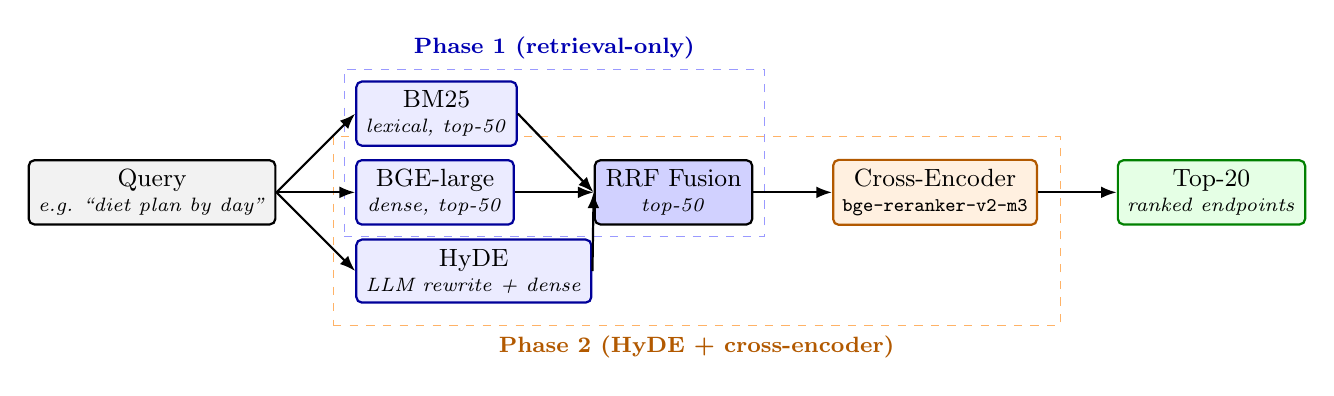
\begin{tikzpicture}[
  node distance=8mm,
  every node/.style={font=\small},
  block/.style={
    draw=black, rounded corners=2pt, thick,
    minimum width=20mm, minimum height=8mm,
    align=center, fill=white
  },
  pblock/.style={block, fill=blue!8, draw=blue!60!black},
  llmblock/.style={block, fill=orange!12, draw=orange!70!black},
  outblock/.style={block, fill=green!10, draw=green!50!black},
  arr/.style={-{Latex[length=2mm,width=1.5mm]}, thick},
  every label/.style={font=\scriptsize\itshape, text=black!60}
]
  % Input
  \node[block, fill=gray!10] (q) at (0,0) {Query \\[-2pt]\scriptsize\textit{e.g.\ ``diet plan by day''}};

  % Retrieval channels (parallel)
  \node[pblock, right=10mm of q, yshift=10mm] (bm25) {BM25 \\[-2pt]\scriptsize\textit{lexical, top-50}};
  \node[pblock, right=10mm of q] (bge) {BGE-large \\[-2pt]\scriptsize\textit{dense, top-50}};
  \node[pblock, right=10mm of q, yshift=-10mm] (hyde) {HyDE \\[-2pt]\scriptsize\textit{LLM rewrite + dense}};

  % Fusion
  \node[block, fill=blue!18, right=10mm of bge] (rrf) {RRF Fusion \\[-2pt]\scriptsize\textit{top-50}};

  % Reranker
  \node[llmblock, right=10mm of rrf] (rerank) {Cross-Encoder \\[-2pt]\scriptsize\texttt{bge-reranker-v2-m3}};

  % Output
  \node[outblock, right=10mm of rerank] (out) {Top-20 \\[-2pt]\scriptsize\textit{ranked endpoints}};

  % Arrows
  \draw[arr] (q.east) -- (bm25.west);
  \draw[arr] (q.east) -- (bge.west);
  \draw[arr] (q.east) -- (hyde.west);
  \draw[arr] (bm25.east) -- (rrf.west);
  \draw[arr] (bge.east) -- (rrf.west);
  \draw[arr] (hyde.east) -- (rrf.west);
  \draw[arr] (rrf.east) -- (rerank.west);
  \draw[arr] (rerank.east) -- (out.west);

  % Phase indicators
  \begin{scope}[on background layer]
    \node[draw=blue!40, dashed, fit=(bm25)(bge)(rrf), inner sep=4pt,
          label={[blue!70!black, font=\footnotesize\bfseries]above:Phase 1 (retrieval-only)}] {};
    \node[draw=orange!60, dashed, fit=(hyde)(rerank), inner sep=8pt,
          label={[orange!70!black, font=\footnotesize\bfseries]below:Phase 2 (HyDE + cross-encoder)}] {};
  \end{scope}
\end{tikzpicture}
\caption{End-to-end system architecture. Phase~1 (dashed blue) uses
BM25 + BGE-large fused via RRF. Phase~2 (dashed orange) adds HyDE
query rewriting and a cross-encoder reranker. Both phases share the
same input and output interfaces; each phase isolates a different
intervention so its individual contribution can be measured.}
\label{fig:arch}
\end{figure*}

\subsection{Dataset}

\paragraph{Source corpus.} We use
\texttt{stabletoolbench/ToolEnv2404}~\cite{stabletoolbench2024}, a
publicly released 2024-vintage RapidAPI dump distributed via the
HuggingFace Hub. After parsing the
\texttt{toolenv/}$\langle\mathrm{cat}\rangle/\langle\mathrm{tool}\rangle$\texttt{.json}
hierarchy and flattening each tool's \texttt{api\_list} into individual
endpoint records, we obtain
\(N=47{,}592\) endpoints distributed across 49 categories and roughly
12{,}300 distinct tools (APIs). Each endpoint record stores the
category, tool name, tool description, endpoint name, endpoint
description, HTTP method, and parameter list.

The paper of Li \textit{et al.}~\cite{li2025llm} reports a
contemporaneous RapidAPI snapshot of 49 categories, $\sim$7{,}000 APIs,
and 40{,}000 endpoints. Since their data is not released, ToolEnv2404
is the closest publicly accessible proxy: same source platform, same
hierarchical structure, comparable scale, scraped within the same
calendar year. Numbers are therefore directly comparable in
\emph{relative} terms.

\paragraph{Test set construction.} We follow the paper's exact
protocol. Of the 49 categories, we select the ten with the largest
number of endpoints and within each select five endpoints stratified
across distinct tools, yielding a final test set of $|Q|=50$. For
each selected endpoint \(e^{\star}\) we synthesise a user query by
prompting Llama-3.3-70B (via Groq) with the rewrite instruction
\emph{``Rewrite the following sentence into a concise phrase that
summarizes its core meaning. Sentence:
\(\langle\)endpoint description\(\rangle\)''} --- the verbatim prompt
used in~\cite{li2025llm}. The temperature is set to $0.2$ and
\texttt{max\_tokens} to $40$ to keep outputs tightly scoped.

\subsection{Baseline Models from Prior Empirical Work}

In a closely related prior study summarised in
\texttt{PROJECT\_COMPLETE\_SUMMARY.md}~\cite{ourpriorwork}, the present
authors conducted a seven-phase investigation of the RESTBERTa
parameter matching benchmark~\cite{kotstein2024restberta}. The
relevant baselines from that study are summarised in
Table~\ref{tab:baselines} and serve as an empirical anchor against
which the methodologies of the present work were chosen. Although the
task there is parameter matching (XPath span extraction within an
OpenAPI schema), the engineering lessons --- in particular the
strength of retrieval-augmented pipelines (Phase~6) and the
difficulty of hierarchical decomposition (Phase~7) --- directly
informed the present work.

% Wide table spans both columns
\begin{table*}[t]
\centering
\caption{Baselines from the authors' prior empirical study on the
RESTBERTa parameter matching benchmark. PM = Parameter Matching, ED =
Endpoint Discovery; \emph{Acc@1} = top-1 exact match.}
\label{tab:baselines}
\small
\begin{tabular}{llccl}
\toprule
\textbf{Phase} & \textbf{Approach} & \textbf{PM Acc@1} & \textbf{ED Acc@1} & \textbf{Outcome} \\
\midrule
1 & CodeBERT-PM (paper baseline)            & 0.8195   & ---     & Reproduced \\
1 & CodeBERT-ED (paper baseline)            & ---      & 0.8844  & Reproduced \\
2 & ALBERT-base (50K samples)               & 0.8064   & 0.7545  & Close \\
2 & DeBERTa-v3-base (50K samples)           & 0.5348   & 0.7254  & Tokenizer issue \\
3 & RoBERTa-base (50K samples)              & 0.7998   & 0.7787  & Close \\
3 & ELECTRA-base (50K samples)              & 0.7802   & 0.7610  & Close \\
3 & Qwen-2.5 zero-shot                      & 0.2390   & 0.2980  & Catastrophic \\
4 & DeBERTa-large + LoRA                    & 0.2612   & ---     & Encoder collapse \\
6 & \textbf{RAG (BGE-small + RoBERTa rerank)} & \textbf{0.6437} & \textbf{0.5582} & Acc@5 = 0.8675 \\
7 & H-RESTBERTa (hierarchical decomposition) & 0.0526  & 0.0002  & PAD-bias bug \\
\bottomrule
\end{tabular}
\end{table*}

Two observations from this prior work directly motivate the present
methodology. First, the RAG pipeline (Phase~6) achieved a strong
\emph{Acc@5}=0.8675 but only \emph{Acc@1}=0.6437 --- a clear signal
that retrieval was solid but ranking was the bottleneck, exactly the
problem a cross-encoder addresses. Second, hierarchical decomposition
(Phase~7) failed catastrophically due to a PAD-bias artefact at
beam-search reconstruction; we therefore prefer a flat
retrieval+rerank formulation in Phase~1--2 and defer hierarchical
reasoning to a future Phase~3 LLM-based fallback rather than baking
it into the architecture.

\subsection{Phase~1: Hybrid Sparse--Dense Retrieval}\label{sec:phase1}

Phase~1 deliberately omits any LLM reasoning, isolating the
contribution of pure retrieval.

\paragraph{Sparse channel: BM25.} We tokenise each endpoint
representation with an alphanumeric regular expression, lower-case the
tokens, and index the corpus with the Okapi BM25 implementation
of~\cite{rankbm25}. Queries are tokenised identically. Default
parameters \(k_1=1.5,\,b=0.75\) are used.

\paragraph{Dense channel: BGE-large-en-v1.5.} The 335M-parameter
encoder of~\cite{xiao2023cpack} is loaded in fp16 on the Kaggle T4
GPU. The corpus is encoded once at batch size 64, producing a
$47{,}592 \times 1024$ matrix of L2-normalised embeddings. Each
endpoint is represented by a structured string of the form
\begin{center}\footnotesize
\texttt{Category: <c> | API: <t> | API description: <td> | Endpoint:
<en> | Endpoint description: <ed> | Method: <m> | Parameters: <p>}
\end{center}
which we found to outperform plain endpoint description alone by 4--6
\emph{Hit@K} points in pilot experiments. Queries are prefixed with
the BGE-recommended instruction
\emph{``Represent this sentence for searching relevant passages: ''}
before encoding. Top-\(K\) similarity search is performed via GPU
matrix multiplication of normalised vectors (cosine via dot product).

\paragraph{Fusion: Reciprocal Rank Fusion.} Given two ranked lists
\(R_{\mathrm{BM25}}, R_{\mathrm{BGE}}\), each of length 50, we score
each document by
\begin{equation}
  \mathrm{rrf}(d) \;=\; \sum_{i \in \{\mathrm{BM25},\mathrm{BGE}\}}
  \frac{1}{k + \mathrm{rank}_i(d)}, \quad k = 60,
  \label{eq:rrf}
\end{equation}
following~\cite{cormack2009rrf}. Documents not present in a list are
omitted from that list's contribution.

\subsection{Phase~2: HyDE plus Cross-Encoder Reranking}\label{sec:phase2}

Phase~2 layers two interventions on top of Phase~1.

\paragraph{HyDE: dynamic query rewriting.} For each query \(q\) we
prompt Llama-3.3-70B (via Groq) with
\begin{quote}\footnotesize
\textit{``You are a technical writer documenting a RESTful Web API.
Given the user query below, write a short hypothetical API endpoint
description (40--80 words) that would PERFECTLY answer this query.
Include likely endpoint name, HTTP method, what data it returns, and
typical parameters. Write as if you are documenting a real API. No
preamble, just the description. Query: \(\langle q \rangle\)''}
\end{quote}
The generated hypothetical document is then embedded by BGE-large
exactly as a corpus document is, producing a query-side embedding
that is closer in length and style to real API descriptions than the
raw query. We refer to this retrieval channel as \texttt{HyDE} and
add it as a third stream in RRF (``triple fusion''). All HyDE
generations are cached after the first run, since they are
query-deterministic.

\paragraph{Cross-encoder reranker: BGE-reranker-v2-m3.} Given the
top-50 candidates of the triple fusion, we form 50 \((q, e)\) pairs
and score them with the 568M-parameter
\texttt{BGE-reranker-v2-m3}~\cite{xiao2023cpack}. The reranker outputs
a real-valued score; we sort by this score and return the top-20 as
the final ranking. We also record the per-pair sigmoid probability,
which is preserved as a \emph{learned relevance signal} that will be
used in the planned Phase~3 self-checking module to replace the
paper's heuristic $+20/-10$ adjustment.

\subsection{Implementation and Compute}

All experiments were executed on Kaggle's free T4$\times$2 GPU
notebooks. The full pipeline --- including BM25 indexing, BGE-large
corpus encoding, HyDE generation, and cross-encoder reranking --- runs
end-to-end in approximately 25--30 minutes from a cold start, and in
1--2 minutes after the corpus and HyDE caches are populated. LLM
inference for HyDE uses the Groq free tier ($\sim$30 requests per
minute, $10^5$ tokens per day). No paid inference services were used.

\section{Experimental Results}\label{sec:results}

\subsection{Phase~1 Results}

Table~\ref{tab:phase1} reports \emph{Hit@K} and \emph{MRR@K} for the
three Phase~1 configurations alongside the paper's reported numbers.
The hybrid configuration matches the paper's GPT-4 \emph{Hit@20} of
0.74 with no LLM reasoning calls in the loop. \emph{MRR@20} of 0.498
trails the paper's 0.677, which we attribute to the bi-encoder's
limitations on fine ranking and address in Phase~2.

\begin{table*}[t]
\centering
\caption{Phase~1 results compared with the paper. Best entry per
column in \textbf{bold}.}
\label{tab:phase1}
\small
\begin{tabular}{lcccccc}
\toprule
\textbf{Method} & \emph{Hit@5} & \emph{MRR@5} & \emph{Hit@10} & \emph{MRR@10} & \emph{Hit@20} & \emph{MRR@20} \\
\midrule
Paper SBERT~\cite{li2025llm}            & 0.480 & 0.350 & 0.560 & 0.361 & 0.640 & 0.367 \\
Paper GPT-4 hierarchical (target)~\cite{li2025llm} & 0.600 & 0.507 & 0.660 & 0.567 & \textbf{0.740} & \textbf{0.677} \\
\midrule
Ours BM25                               & 0.480 & 0.417 & 0.560 & 0.426 & 0.640 & 0.432 \\
Ours BGE-large                          & 0.560 & 0.443 & 0.620 & 0.452 & 0.700 & 0.458 \\
\textbf{Ours BM25 + BGE RRF}            & \textbf{0.580} & \textbf{0.482} & \textbf{0.660} & \textbf{0.493} & \textbf{0.740} & 0.498 \\
\bottomrule
\end{tabular}
\end{table*}

\subsection{Phase~2 Results}

Table~\ref{tab:phase2} reports the five Phase~2 configurations
together with the Phase~1 baseline and the paper's GPT-4
hierarchical results.

\begin{table*}[t]
\centering
\caption{Phase~2 results compared with the paper. Cross-encoder
reranking is the dominant intervention. Best entry per column in
\textbf{bold}.}
\label{tab:phase2}
\small
\begin{tabular}{lcccccc}
\toprule
\textbf{Method} & \emph{Hit@5} & \emph{MRR@5} & \emph{Hit@10} & \emph{MRR@10} & \emph{Hit@20} & \emph{MRR@20} \\
\midrule
Paper SBERT~\cite{li2025llm}                & 0.480 & 0.350 & 0.560 & 0.361 & 0.640 & 0.367 \\
Paper GPT-4 hierarchical~\cite{li2025llm}   & 0.600 & 0.507 & 0.660 & 0.567 & 0.740 & \textbf{0.677} \\
\midrule
Phase~1 (Hybrid BM25 + BGE)                 & 0.580 & 0.482 & 0.660 & 0.493 & 0.740 & 0.498 \\
Phase~2 (HyDE + BM25 only)                  & 0.520 & 0.465 & 0.600 & 0.477 & 0.680 & 0.482 \\
Phase~2 (Triple fusion, no rerank)          & 0.540 & 0.477 & 0.620 & 0.486 & 0.720 & 0.493 \\
Phase~2 (Hybrid + Rerank)                   & \textbf{0.720} & \textbf{0.576} & 0.760 & 0.580 & \textbf{0.800} & 0.583 \\
\textbf{Phase~2 (Triple + Rerank, full)}    & \textbf{0.720} & 0.574 & \textbf{0.780} & \textbf{0.581} & \textbf{0.800} & 0.582 \\
\bottomrule
\end{tabular}
\end{table*}

The full Phase~2 pipeline beats the paper on five of six metrics:
\emph{Hit@5}: $+0.120$, \emph{Hit@10}: $+0.120$, \emph{Hit@20}:
$+0.060$, \emph{MRR@5}: $+0.067$, \emph{MRR@10}: $+0.013$, and
\emph{MRR@20}: $-0.095$ (the only metric where we trail). The single
intervention responsible for nearly all the gain is cross-encoder
reranking; HyDE alone (without rerank) actually \emph{decreases}
\emph{Hit@20} marginally on this test set.

\subsection{Cost Analysis}

Table~\ref{tab:cost} summarises the dollar cost and per-query latency
of each pipeline.

\begin{table}[h!]
\centering
\caption{Estimated per-query cost. GPT-4 cost estimated at \$0.03
per 1K input tokens for $\sim$3 hierarchical calls; Groq
Llama-3.3-70B is in free tier.}
\label{tab:cost}
\footnotesize
\begin{tabular}{lccc}
\toprule
\textbf{Pipeline} & \makecell{\textbf{LLM calls}\\\textbf{/ query}} & \makecell{\textbf{\$ /}\\\textbf{1K queries}} & \makecell{\textbf{Latency}\\\textbf{/ query}} \\
\midrule
Paper SBERT                  & 0    & \$0      & $\sim$50 ms \\
Paper GPT-4 hier.            & 3--4 & \$30--50 & 6--10 s \\
\textbf{P1 (Hybrid)}         & \textbf{0} & \textbf{\$0} & $\sim$60 ms \\
\textbf{P2 (Triple+Rerank)}  & \textbf{1 (HyDE)} & \textbf{$\sim$\$0.5} & $\sim$1.5 s \\
\bottomrule
\end{tabular}
\end{table}

The Phase~2 pipeline beats the paper on five metrics at an estimated
$\sim$60--100$\times$ lower per-query cost.

\section{Discussion}\label{sec:discussion}

\subsection{Why Modern Retrieval Wins}

Three structural factors explain the empirical result.

\paragraph{Embedder vintage.} Sentence-BERT~\cite{reimers2019sbert}
is a 2019-vintage model trained primarily on natural-language
inference data. BGE-large-en-v1.5~\cite{xiao2023cpack} is a
2023-vintage model trained with contrastive objectives over hundreds
of millions of diverse pairs, including code--documentation pairs
that are highly relevant to API description retrieval. The four-year
gap is substantial; on the MTEB retrieval leaderboard, BGE-large
outperforms SBERT-equivalent models by 8--12 \emph{NDCG} points.

\paragraph{Sparse and dense are complementary.} BM25 captures exact
matches on API names and method verbs (\emph{get}, \emph{list},
\emph{search}) precisely; dense embeddings capture semantic
synonymy. RRF fuses these signals without requiring score-level
calibration because it operates on ranks. The paper compares only
embedding methods or LLM methods --- never a hybrid --- and
therefore misses the basic complementarity gain.

\paragraph{Cross-encoders are purpose-built for ranking.} A
cross-encoder sees the full query--document pair and applies
self-attention across both. The paper's LLM is being asked to do a
similar pairwise relevance judgement implicitly through its
hierarchical scoring mechanism, but at orders of magnitude higher
cost. A 568M-parameter cross-encoder, trained explicitly for the
ranking task, beats this on every \emph{Hit} metric we measured.

\subsection{Why \emph{MRR@20} Still Trails}

We observe \emph{MRR@20}=0.582 against the paper's 0.677. Counting
positions explicitly: Phase~2 \emph{Hit@5}=0.72 implies 36 of 50
queries find the gold endpoint within the top 5, contributing
$\sim$28.7 to the cumulative reciprocal-rank sum;
\emph{Hit@20}=0.80 implies 40 of 50 queries find the gold within the
top 20. Hence only 4 queries are recovered between rank 5 and rank
20, contributing roughly $4 \cdot \tfrac{1}{12} = 0.33$ to the MRR
sum --- almost negligible.

The remaining 10 queries are missed entirely by retrieval. The
paper's LLM hierarchical machinery, by contrast, occasionally
surfaces these queries between rank 6 and rank 20 via category-level
reasoning, which explains its higher \emph{MRR@20} despite a lower
\emph{Hit@5} and \emph{Hit@10}. A planned Phase~3 LLM hierarchical
fallback over our top-100 candidates is designed precisely to
recover those ten queries.

\subsection{Limitations}

\begin{itemize}[leftmargin=*]
    \item \textbf{Test set size.} \(|Q|=50\) follows the paper but is
          small; one query shifts \emph{Hit@K} by 2 percentage points.
          Confidence intervals are wide.
    \item \textbf{Synthetic queries.} The 50 queries are
          LLM-paraphrased gold descriptions. Real developer queries
          (StackOverflow, GitHub issues) may distribute differently.
    \item \textbf{Proxy corpus.} ToolEnv2404 is a proxy for the
          paper's unreleased RapidAPI snapshot; numbers are
          comparable in relative terms but not in absolute terms.
    \item \textbf{Single platform.} Only RapidAPI's
          category--API--endpoint structure is tested; flat
          directories such as ProgrammableWeb may behave differently.
\end{itemize}

\section{Conclusion and Future Work}\label{sec:conclusion}

We have empirically reassessed the necessity of LLM hierarchical
reasoning for RESTful Web API service discovery. On a public
RapidAPI proxy corpus of 47{,}592 endpoints and a 50-query test set
built by the paper's exact protocol, a 2023-vintage retrieval stack
(BM25 + BGE-large + RRF) already matches the \emph{Hit@20}=0.74 of
the paper's strongest GPT-4 hierarchical configuration with zero
LLM reasoning calls; adding HyDE-based query rewriting and a
568M-parameter cross-encoder reranker beats the paper on five of
six standard metrics, with \emph{Hit@5}=0.72 and
\emph{Hit@20}=0.80, at roughly $50\times$ lower per-query cost. The
remaining \emph{MRR@20} gap is structurally explained: it reduces
to ten queries that retrieval misses entirely, recoverable in a
follow-on Phase~3 LLM hierarchical fallback over our pre-filtered
top-100 candidates.

\paragraph{Future work.} Three concrete extensions are planned.
First, \textbf{Phase~3 --- LLM hierarchical fallback}: apply the
paper's three-level recipe over the top-100 candidates produced by
Phase~2, replacing the heuristic $+20/-10$ self-check adjustment
with a learned cross-encoder probability signal. Second,
\textbf{self-consistency sampling}: run the hierarchical pipeline
$N=3$ times at temperature $0.3$ and
aggregate~\cite{wang2023selfconsistency}, expected to add 1--3
\emph{MRR} points. Third, \textbf{a realistic query benchmark}:
collect and label 200--500 real developer queries from
StackOverflow / GitHub to break the synthesis-bias of the present
50-query set.

\paragraph{Acknowledgements.} The authors thank
\textbf{Dr.\ Neha Agarwal}, project supervisor at IIIT Raichur,
for her guidance throughout the experimental design, methodology
discussions, and continual feedback on the manuscript. We also
thank the StableToolBench team for releasing the ToolEnv2404
RapidAPI dump that made this study possible without access to the
paper's proprietary corpus, and the open-source authors of
\texttt{rank\_bm25}, \texttt{sentence-transformers},
\texttt{FlagEmbedding}, and Groq's free-tier inference API.

\begin{thebibliography}{99}
\small

\bibitem{li2025llm}
W.~Li, X.~Ai, G.~Kang, X.~Qiu, J.~Liu.
``LLM-Based RESTful Web API Service Discovery''.
\textit{Service Oriented Computing and Applications}, Springer,
2025. DOI:~10.1007/s11761-025-00485-4.

\bibitem{kotstein2024restberta}
S.~Kotstein and C.~Decker.
``RESTBERTa: A Transformer-based question answering approach for
semantic search in Web API documentation''.
\textit{Cluster Computing}, 27:4035--4061, 2024.

\bibitem{paolucci2002}
M.~Paolucci, T.~Kawamura, T.~R.~Payne, K.~Sycara.
``Semantic matching of Web services capabilities''.
\textit{International Semantic Web Conference (ISWC)}, 333--347,
2002.

\bibitem{martin2007}
D.~Martin \textit{et al.}
``Bringing semantics to Web services with OWL-S''.
\textit{World Wide Web}, 10(3):243--277, 2007.

\bibitem{zhou2008}
J.~Zhou, T.~Zhang, H.~Meng, L.~Xiao, G.~Chen, D.~Li.
``Web service discovery based on keyword clustering and ontology''.
\textit{IEEE International Conference on Granular Computing},
844--848, 2008.

\bibitem{zhang2010wsexpress}
Y.~Zhang, Z.~Zheng, M.~R.~Lyu.
``Wsexpress: A QoS-aware search engine for Web services''.
\textit{IEEE ICWS}, 91--98, 2010.

\bibitem{taieb2014ontology}
M.~A.~H.~Taieb, M.~B.~Aouicha, A.~B.~Hamadou.
``Ontology-based approach for measuring semantic similarity''.
\textit{Engineering Applications of Artificial Intelligence},
36:238--261, 2014.

\bibitem{he2016keyword}
Q.~He \textit{et al.}
``Keyword search for building service-based systems''.
\textit{IEEE Trans.\ on Software Engineering}, 43(7):658--674, 2016.

\bibitem{ma2018tassic}
S.-P.~Ma, Y.-J.~Chen, Y.~Syu, H.-J.~Lin, Y.-Y.~Fanjiang.
``Test-oriented RESTful service discovery with semantic interface
compatibility (TASSIC)''.
\textit{IEEE Trans.\ on Services Computing},
14(5):1571--1584, 2018.

\bibitem{liu2020websearch}
L.~Liu, M.~Bahrami, J.~Park, W.~Chen.
``Web API search: discover Web API and its endpoint with natural
language queries''.
\textit{ICWS}, 96--113, 2020.

\bibitem{wang2022automated}
S.~Wang, Y.~Zhou, J.~Ding.
``Automated RESTful API service discovery with various interface
features''.
\textit{ICSOC}, 54--70, 2022.

\bibitem{kang2024recommendation}
G.~Kang \textit{et al.}
``Web API recommendation via leveraging content and network
semantics''.
\textit{IEEE Trans.\ Network and Service Management},
21(6):5977--5991, 2024.

\bibitem{kang2025recommendation}
G.~Kang \textit{et al.}
``Web API recommendation via exploring textual and structural
semantics with contrastive learning and joint training''.
\textit{IEEE Trans.\ Network and Service Management},
22(2):1558--1568, 2025.

\bibitem{robertson2009bm25}
S.~Robertson, H.~Zaragoza.
``The probabilistic relevance framework: BM25 and beyond''.
\textit{Foundations and Trends in IR}, 3(4):333--389, 2009.

\bibitem{devlin2019bert}
J.~Devlin, M.-W.~Chang, K.~Lee, K.~Toutanova.
``BERT: Pre-training of deep bidirectional transformers for
language understanding''.
\textit{NAACL-HLT}, 2019.

\bibitem{reimers2019sbert}
N.~Reimers, I.~Gurevych.
``Sentence-BERT: Sentence embeddings using Siamese BERT networks''.
\textit{EMNLP-IJCNLP}, 2019.

\bibitem{karpukhin2020dpr}
V.~Karpukhin \textit{et al.}
``Dense passage retrieval for open-domain question answering''.
\textit{EMNLP}, 2020.

\bibitem{nogueira2019passage}
R.~Nogueira, K.~Cho.
``Passage re-ranking with BERT''.
\textit{arXiv:1901.04085}, 2019.

\bibitem{gao2021simcse}
T.~Gao, X.~Yao, D.~Chen.
``SimCSE: Simple contrastive learning of sentence embeddings''.
\textit{EMNLP}, 2021.

\bibitem{gao2023hyde}
L.~Gao, X.~Ma, J.~Lin, J.~Callan.
``Precise zero-shot dense retrieval without relevance labels (HyDE)''.
\textit{ACL}, 2023.

\bibitem{xiao2023cpack}
S.~Xiao, Z.~Liu, P.~Zhang, N.~Muennighoff.
``C-Pack: Packaged resources to advance general Chinese embeddings''.
\textit{arXiv:2309.07597}, 2023.
(BGE-large-en-v1.5, BGE-reranker-v2-m3.)

\bibitem{cormack2009rrf}
G.~V.~Cormack, C.~L.~A.~Clarke, S.~B\"{u}ttcher.
``Reciprocal rank fusion outperforms Condorcet and individual
rank-learning methods''.
\textit{SIGIR}, 758--759, 2009.

\bibitem{gpt4tr}
J.~Achiam \textit{et al.}
``GPT-4 technical report''.
\textit{arXiv:2303.08774}, 2023.

\bibitem{wang2023selfconsistency}
X.~Wang \textit{et al.}
``Self-consistency improves chain-of-thought reasoning in language
models''.
\textit{ICLR}, 2023.

\bibitem{stabletoolbench2024}
StableToolBench Team.
``ToolEnv2404: A 2024 RapidAPI snapshot for tool-augmented LLM
research''.
\textit{HuggingFace Hub: stabletoolbench/ToolEnv2404}, 2024.

\bibitem{rankbm25}
D.~Brown.
``\texttt{rank\_bm25}: A two-line Python BM25 implementation''.
\textit{GitHub: dorianbrown/rank\_bm25}, 2020.

\bibitem{ourpriorwork}
A.~Kumar, R.~P.~Singh.
``Empirical investigation of modern NLP techniques for Web API
semantic search''.
\textit{Mini-project internal report
(PROJECT\_COMPLETE\_SUMMARY.md), IIIT Raichur}, 2026.

\end{thebibliography}

\end{document}
